\subsection{Boundary Scores PCA}\label{HiC:boundary-scores-pca}% __10b-boundary-scores-pca
%~~~~~~~~~~~~~~~~~~~%
\subsubsection{Input} % inputs
Data from the pipeline \texttt{boundary-scores} step is used as input (Section~\ref{HiC:boundary-scores}).
%~~~~~~~~~~~~~~~~~~~%
\subsubsection{Analysis} % analysis
Default parameters:
\begin{lstlisting}
params.standard.tcsh
#!/bin/tcsh

source ./inputs/params/params.tcsh

set chrom_excluded = 'chr[MYX]'              # excluded chromosomes

set group_var = 'cell_type'                  # grouping variable (from sample sheet) to be used for color assignment)
\end{lstlisting}
%~~~~~~~~~~~~~~~~~~~%
\subsubsection{Output} % outputs
See Figure~\ref{fig:boundary-scores-pca_DI_k_001}. Default output: %results/boundary-scores-pca.standard/boundary-scores.by_sample.standard/matrix-filtered.by_sample.res_40kb/filter.by_sample.standard/align.by_sample.bowtie2/hg19/all-samples/
\begin{lstlisting}
-rw-r--r-- 1 at570 4.1K Feb 15 15:20 job.err
-rw-r--r-- 1 at570   47 Feb 15 15:18 job.id
-rw-r--r-- 1 at570  936 Feb 15 15:20 job.out
-rw-r--r-- 1 at570  564 Feb 15 15:18 job.sh
-rw-r--r-- 1 at570 4.8K Feb 15 15:20 job.vars.tsv
-rw-r--r-- 1 at570  211 Feb 15 15:18 labels.tsv
-rw-r--r-- 1 at570 4.4K Feb 15 15:19 pca.DI.k=001.pdf
-rw-r--r-- 1 at570 4.4K Feb 15 15:19 pca.DI2.k=001.pdf
-rw-r--r-- 1 at570 4.4K Feb 15 15:19 pca.diff.k=001.pdf
-rw-r--r-- 1 at570 4.4K Feb 15 15:20 pca.diffratio.k=001.pdf
-rw-r--r-- 1 at570 4.4K Feb 15 15:19 pca.inter.k=001.pdf
-rw-r--r-- 1 at570 4.4K Feb 15 15:18 pca.intra-left.k=001.pdf
-rw-r--r-- 1 at570 4.4K Feb 15 15:19 pca.intra-max.k=001.pdf
-rw-r--r-- 1 at570 4.4K Feb 15 15:19 pca.intra-min.k=001.pdf
-rw-r--r-- 1 at570 4.4K Feb 15 15:18 pca.intra-right.k=001.pdf
-rw-r--r-- 1 at570 4.4K Feb 15 15:20 pca.novel-max.k=001.pdf
-rw-r--r-- 1 at570 4.4K Feb 15 15:20 pca.novel-min.k=001.pdf
-rw-r--r-- 1 at570 4.4K Feb 15 15:19 pca.ratio.k=001.pdf
\end{lstlisting}

% \begin{figure}[!h]%!htb
\begin{figure}[!htb]%
    \centering
    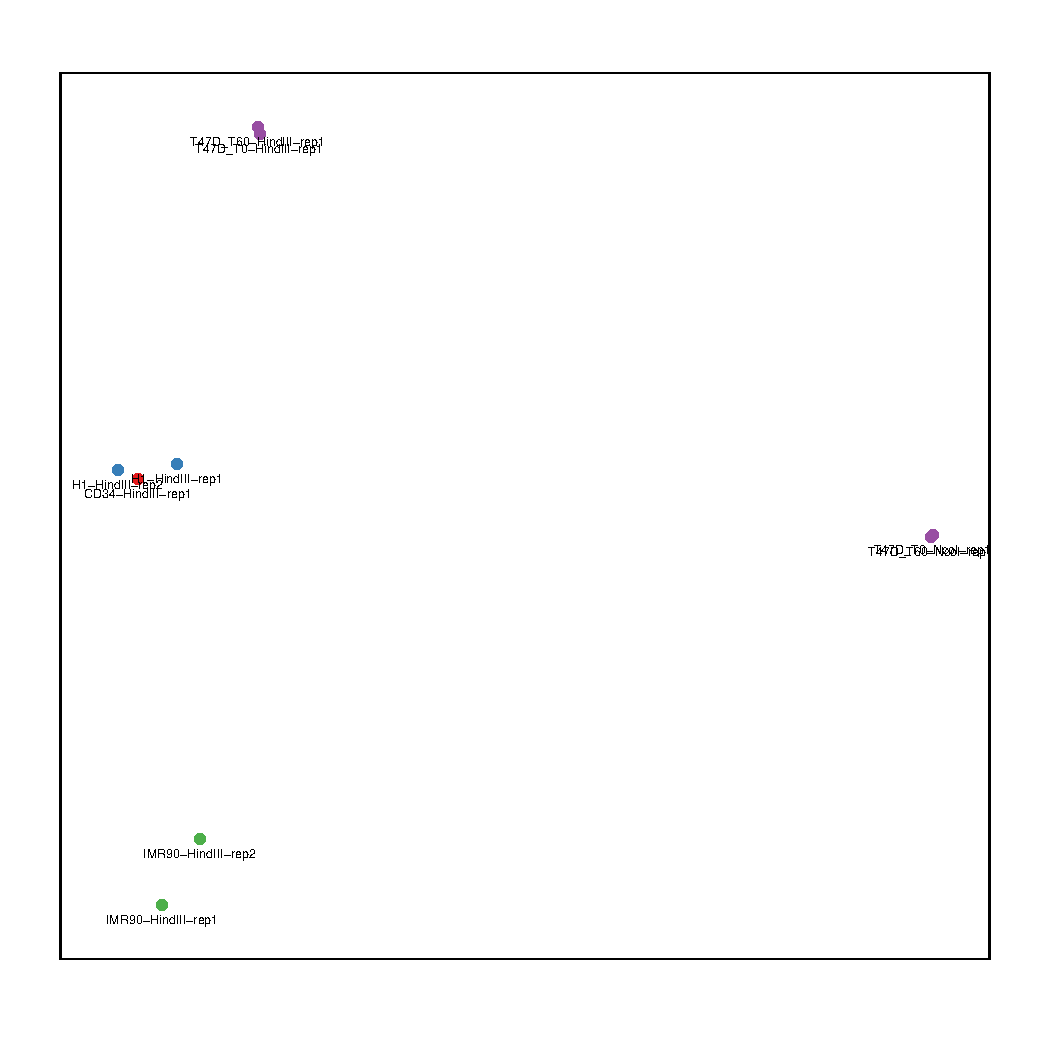
\includegraphics[width=\textwidth,height=\textheight,keepaspectratio]{figure/boundary-scores-pca_pca_DI_k_001}
    \caption{Boundary Scores PCA sample output. See Section~\ref{HiC:boundary-scores-pca}.} % results/boundary-scores-pca.standard/boundary-scores.by_sample.standard/matrix-filtered.by_sample.res_40kb/filter.by_sample.standard/align.by_sample.bowtie2/hg19/all-samples/pca.DI.k=001.pdf
    \label{fig:boundary-scores-pca_DI_k_001}
\end{figure}
% \newpage
\clearpage